Eingereicht:

\begin{verbatim}[1, 3]\end{verbatim}

Gewählte Option 1 ist verfügbar?\begin{quote}Yes.\end{quote}Gewählte Option 3 ist verfügbar?\begin{quote}Yes.\end{quote}Anmerkungen zur eingereichten Lösung:

Alle angegebenen Klassendiagramme sind korrekt?

\begin{quote}\begin{verbatim}Nein.\end{verbatim}\end{quote}

Die korrekte Lösung ist:\begin{verbatim}[1,4]\end{verbatim}

Ihre Antwort zu Klassendiagramm 3 ist nicht richtig.

Klassendiagramm 3 ist ungültig.

Die Beziehungen in dem Klassendiagramm könnten auf folgende Weise mit Namen versehen werden:



\begin{centering}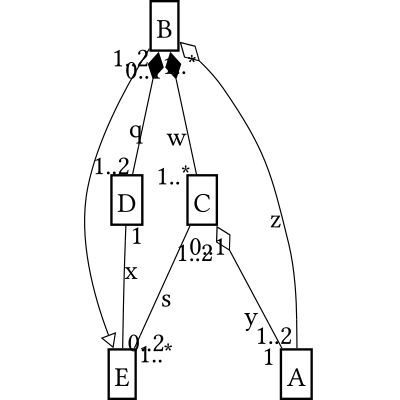
\includegraphics[min width=0.4\textwidth=0.6\textwidth,min height=0.4\textwidth=0.6\textwidth,keepaspectratio,max width=0.9\textwidth,max height=0.9\textwidth]{52/cdbb94aeaa70e6e2bba23762be906eba6c07a58494f0038c6902b3ecf93df0d24201af83b04c596701db35357ce8aed00a3a92e08161.pdf}\end{centering}



Wenn es zum Beispiel Komposition q nicht gäbe, wäre es gültig.

Ihre Antwort zu Klassendiagramm 4 ist nicht richtig.

Klassendiagramm 4 ist gültig.

Die Beziehungen in dem Klassendiagramm könnten auf folgende Weise mit Namen versehen werden:



\begin{centering}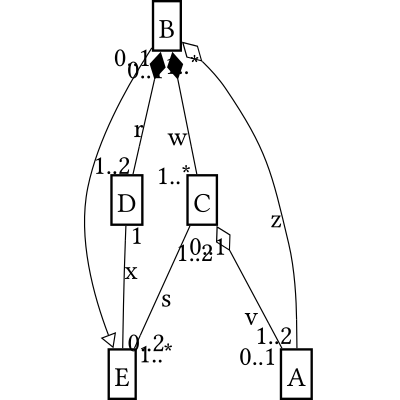
\includegraphics[min width=0.4\textwidth=0.6\textwidth,min height=0.4\textwidth=0.6\textwidth,keepaspectratio,max width=0.9\textwidth,max height=0.9\textwidth]{52/cdd98fa5f9699f7f24fc7953cf62b89e3298c6ff397cc23315cb8f3389b466b03201af83b04c596701db35357ce8aed00a3a92e08161.pdf}\end{centering}



Betrachten Sie nun das folgende Objektdiagramm, welches eine Instanz dieses Klassendiagramms ist:



\begin{centering}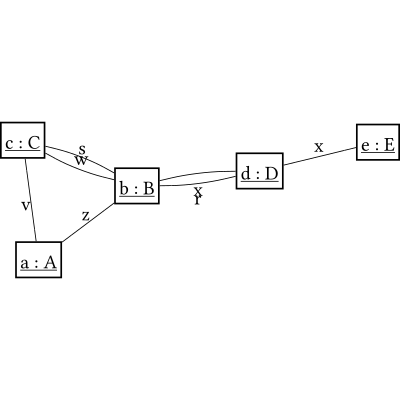
\includegraphics[min width=0.4\textwidth=0.6\textwidth,min height=0.4\textwidth=0.6\textwidth,keepaspectratio,max width=0.9\textwidth,max height=0.9\textwidth]{52/odb3dd8f1d0590ffb74d7617dd795cf3342662f4976d2517c3ac02a7745796030013.pdf}\end{centering}



